% --------------------------------------------------------------------
% Preamble
% --------------------------------------------------------------------
\documentclass[paper=a4, fontsize=11pt]{scrartcl}	% KOMA

\usepackage[a4paper,pdftex]{geometry}	% A4paper margins
\setlength{\oddsidemargin}{5mm}			% Remove 'twosided' indentation
\setlength{\evensidemargin}{5mm}

\usepackage{listings}
\lstset{
  basicstyle=\ttfamily\scriptsize,
  mathescape
}
\usepackage{color}
%Code settings
\lstset{
  keywordstyle=\color{blue},
  frame = single,
  numbers = left,
  stepnumber = 5,
  caption=\lstname
}

\usepackage{hyperref}
\usepackage{seqsplit}
\usepackage[us]{datetime}
\usepackage[protrusion=true,expansion=true]{microtype}	
\usepackage{CJKutf8}
\usepackage[utf8]{inputenc}
\usepackage[T1]{fontenc}
\usepackage{amsmath,amsfonts,amsthm,amssymb}
\usepackage{graphicx}
\usepackage{adjustbox}
\usepackage{url}
\usepackage{wrapfig}
\usepackage{lipsum}
\usepackage{titlesec}
\usepackage{float}
% \titleformat{\subsection}

% --------------------------------------------------------------------
% Definitions (do not change this)
% --------------------------------------------------------------------
\newcommand{\HRule}[1]{\rule{\linewidth}{#1}} 	% Horizontal rule

\makeatletter							% Title
\def\printtitle{%						
    {\centering \@title\par}}
\makeatother									

\makeatletter							% Author
\def\printauthor{%					
    {\centering \large \@author}}				
\makeatother							

% --------------------------------------------------------------------
% Metadata (Change this)
% --------------------------------------------------------------------
\title{						% Upper rule
			\LARGE \textbf{\uppercase{HackUPC: The Game}\\Solutions}	% Title
			\HRule{2pt} \\ [0.5cm]		% Lower rule + 0.5cm spacing
			\normalsize \today			% Todays date
		}

\author{
		\textbf{\large{Albert Martínez}}\\[0.3cm]
}


\begin{document}
% ------------------------------------------------------------------------------
% Maketitle
% ------------------------------------------------------------------------------
\thispagestyle{empty}		% Remove page numbering on this page

\printtitle					% Print the title data as defined above
  	\vfill
\printauthor				% Print the author data as defined above
\newpage
% ------------------------------------------------------------------------------
% Begin document
% ------------------------------------------------------------------------------	
\tableofcontents 			%això genera l'index, latex is awesome

\newpage

\section{Special Thanks}
Special thanks go to all organizers from HackUPC that helped to create \texttt{The Game}, specially:
\begin{itemize}
\item Darío Nieuwenhuis and Dani Torramilans, for creating the awesome website.
\item Miquel Llobet, Bernat Moix, Sergio Rodríguez and Antoni Virós, for collaborating in the problemset.
\item Darío Nieuwenhuis, Gerard Orriols and Albert Vaca, for finding errors in the official solution during the contest.
\end{itemize}


\clearpage
\section{Solutions}
Here is the report with solutions for each problem from \texttt{The Game}. Some problems allowed different approaches to solve them. We saw people solving some problems in a clever way we did not expect. Here we show our proposed solutions.

All code with solutions is available at: \url{https://github.com/albertnez/the-game/}.



% \clearpage
\addcontentsline{toc}{subsection}{Level 0: The Game}
\subsection*{Level 0: The Game}
\textit{What did you just lose?}

This is a reference to \textbf{The Game}. Therefore, the answer is \texttt{thegame}.
We made it explicit in the beginning that no answer would contain spaces or capital letters. Of course this didn't stop people from attempting to use them in the first problem, causing confusion.
\\
\\
The answer is \texttt{thegame}.



% \clearpage
\addcontentsline{toc}{subsection}{Level 1: Messy folders}
\subsection*{Level 1: Messy folders}
We are given a \href{https://game.hackupc.com/static/files/messy-folders.zip}{file}, which contains a lot of nested folders with lots of files. We are asked to find the password.

Instead of looking file by file, we can use \texttt{grep -r 'password'}, which will look for the string \textit{password} in all files and subdirectories. With this we find that it matches with \texttt{password=1337p455w0rd}. During the contest we gave the hint to use grep to help contestants.
\\
\\
The answer is \texttt{1337p455w0rd}.



% \clearpage
\addcontentsline{toc}{subsection}{Level 2: Decoding}
\subsection*{Level 2: Decoding}
We are given a text and we are asked to find the password. The title suggests decoding the string, and the string is composed of hexadecimal characters only. If we decode the hex string, we find the next string:

\texttt{WkRGbE5UYzJZamN4WTJObFpqVTVOemhrTWpJeFptRmtaalJtTUdVeU9Ea2dJQzBLCg==}.

As it ends with \texttt{==}, this happens in base64 strings, so we decode base64 and find yet another string:

\texttt{ZDFlNTc2YjcxY2NlZjU5NzhkMjIxZmFkZjRmMGUyODkgIC0K}. 

This string does not give much information how to decode it. However, we could just try to do what we have already done. This is not a hex string, so we just try to decode as a base64 string to find the last string:

\texttt{d1e576b71ccef5978d221fadf4f0e289}.

It has 32 characters, and it is a md5 hash of the password. If we just try to look for that string in Google (or any other search engine), we easily find the original text in of the many MD5 lookup websites, and that is the password.
\\
\\
The answer is \texttt{superpassword}.



\subsection*{Level 3: XOR}
\textit{Somebody did the XOR of all numbers from 0 to 1000000000 (inclusive), except one number K. Find this K.}

We know that $a \oplus a = 0$. So if we apply the XOR of all numbers in the range to the given number, each one will be canceled, except K, that only appears once. Therefore we are left with the original number K. As 1000000000 is not that big, we can do the XOR of all numbers one by one in less than one second.
\\
\\
The answer is \texttt{133333337}.



\addcontentsline{toc}{subsection}{Level 4: TAR}
\subsection*{Level 4: TAR}
We are given a lot of nested compressed files, numbered starting at 512. A simple script can automatically extract everything until we get with the password, as shown in listing \ref{lst:level4}. Some contestants solved by clicking on the file in a DE that automatically displayed the contents inside. We just did not expect anyone to manually open 512 files, but it worked.
\\
\\
The answer is \texttt{aaronswartz}.
\lstinputlisting[language=Python, firstnumber=1, breaklines=true, label={lst:level4}]{code/level4.py}


\addcontentsline{toc}{subsection}{Level 5: Weak die fast}
\subsection*{Level 5: Weak die fast}
We are given a password protected zip file. The password is inside. Here the title suggests that the password is weak, and it is fast to crack. Using an already existing software to crack zips or creating a small script that would try all combinations would find that the password of the zip is \texttt{sat}. A sample script for the task is given in listing \ref{lst:level5}.
\\
\\
The answer is \texttt{knuthmorrispratt}.
\lstinputlisting[language=Python, firstnumber=1, breaklines=true, label={lst:level5}]{code/level5.py}


\addcontentsline{toc}{subsection}{Level 6: Colors}
\subsection*{Level 6: Colors!}
We are given a HackUPC logo and are asked to find the password. Looking carefully at the picture, we could see that some pixels differ from others by 1 value of alpha. If we binarize this image based on that, we obtain a Qr. All this could be done via code, or just with GIMP or any other image editing software for example. Scanning this Qr yields to... another Qr! Scanning this last Qr yields to the password. In listing \ref{lst:level6} there is a simple script to generate the Qr from the image.
\\
\\
The answer is \texttt{kolmogorov}.
\lstinputlisting[language=Python, firstnumber=1, breaklines=true, label={lst:level6}]{code/level6.py}




\addcontentsline{toc}{subsection}{Level 7: Game of Life}
\subsection*{Level 7: Game of Life}
\textit{You are given an initial Game of Life pattern as a matrix of 1s (alive cells) and 0s (dead cells). Calculate the iteration at which the cycle starts, and the length of it. Your solution should of the form (steps\_to\_cycle)-(cycle\_length), without parenthesis. Keep in mind, that this Game of Life uses a looping matrix!}

This can be solved by implementing a game of life, and at each step storing the board in a key-value structure, where the board is the key, and the value is the current iteration number. At some point, we will get to a state that it was already visited. As we know when was first seen, and the current iteration, we can get when it started, and the cycle length with a simple subtraction. There is a C++ sample code in listing \ref{lst:level7}.
\\
\\
The answer is \texttt{286-168}.

\lstinputlisting[language=C++, firstnumber=1, label={lst:level7}]{code/level7.cc}




\addcontentsline{toc}{subsection}{Level 8: There's more than what you see}
\subsection*{Level 8: There's more than what you see}
We are given a link to \url{http://46.101.102.224}, but if we go there, we only see the text \texttt{Hello, this file has nothing for you...}. If we use the hint given in the title, and we look inside the headers, we can see that the response header includes an attribute for the password, as shown in figure \ref{header}.
\\
\\
The answer is \texttt{mllobetisawesome}.

\begin{figure}[H]
\centering
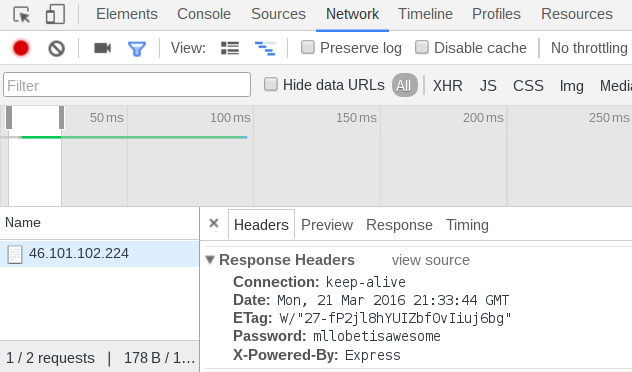
\includegraphics[width=\textwidth]{images/header.png}
\caption{Response header.}
\label{header}
\end{figure}

\addcontentsline{toc}{subsection}{Level 9: Add them all!}
\subsection*{Level 9: Add them all!}
This problem contained lots of images with binary numbers. The solution was to add all numbers in binary and give it in base 10. To solve this problem one could use any OCR software, such as \textit{tesseract}. There is a sample solution in python in listing \ref{lst:level9}.
\\
\\
The answer is \texttt{2601850323}.

\lstinputlisting[language=Python, breaklines=True, firstnumber=1, label={lst:level9}]{code/level9.py}

\addcontentsline{toc}{subsection}{Level 10: Counting bits}
\subsection*{Level 10: Counting bits}
It's easier to count the number of bits from 0 to n. Then we can count from 0 to 1333333333333337, and subtract the amount from 0 to 1337-1 using inclusion exclusion principle. To count from 0 to n, we can use some observations. When $n$ is $2^{i}-1$, we have been through $2^i$ numbers from 0, and each bit to the right of the i-th bit, has been to '1' half of the times. Therefore, each bit has been to '1' exactly $2^{i-1}$ times.

We can iterate through all bits from the left, and keep adding using that observation, whenever there is a bit to '1', we add that one bit, we add the bits to the right for that bit to be '1', and then we continue as if this bit no longer exists. There is a sample code C++ in listing  \ref{lst:level10}. 
\\
\\
The answer is \texttt{33254528318498418}.

\lstinputlisting[language=C++, firstnumber=1, label={lst:level10}]{code/level10.cc}

\addcontentsline{toc}{subsection}{Level 11: Getting inside}
\subsection*{Level 11: Getting inside}
In this problem, we were asked to get inside Linus' server. We were given his private key, username, and the ip of his server. However, if we tried to connect into it via ssh we find a problem:
\begin{verbatim}
$ ssh -i linus_rsa linus@46.101.102.228        
Permission denied (publickey).
\end{verbatim}

Something is wrong here, but all the given data is correct. One could try to use ssh over different ports. Here, due to the number of previous references to 1337, it would make sense to try port 1337. Another way to realize this is to use nmap to search of opened ports. The problem is that nmap does not scan port 1337 by default, but if we give a fairly large range of ports to scan, it will find it.

\begin{verbatim}
$ nmap 46.101.102.228 -p1-2000
Starting Nmap 7.10 ( https://nmap.org ) at 2016-03-22 16:41 CET
Nmap scan report for 46.101.102.228
Host is up (0.078s latency).
Not shown: 1996 closed ports
PORT     STATE    SERVICE
22/tcp   open     ssh
1337/tcp open     waste
\end{verbatim}

Now, trying to ssh using port 1337 does not show us the previous error. In fact, we find that the terminal is cleared and then the connection is closed. If we ssh redirecting the output to a file, this time the content is not deleted, and we get the password. What happened, is that the server by default printed a text file that contained the password with the command \texttt{more}, and then it closed the connection. As the text in the file is fairly small, the command \texttt{more} terminated immediately. If we resize the terminal window to make it smaller, and try again, we see that this time the command \texttt{more} does not finish, as there is not enough space to show all text, and we can see the password as well.
\\
\\
The answer is \texttt{thecakeisalie}.

\addcontentsline{toc}{subsection}{Level 12: XOR Part 2}
\subsection*{Level 12: XOR Part 2}
It is the same problem as Level 3, but this time numbers are to large to XOR all numbers. As there is a previous Level that involves counting the number of bits, we know from that problem that for any $n > 1$, the number of times that each bit has been to '1' from 0 to $2^n$ (exclusive) is even, therefore the XOR is 0. If we try to find a power of two close to the number in the input, we see that $2^{60} = 1152921504606846976$. Since the accumulated XOR to that point is 0, and the amount of numbers from that to the limit from the input is very small, we can do the XOR of the remaining numbers one by one. 

A simpler way to solve this problem, is to realize that the accumulated XOR follows a pattern. Every 4 numbers it becomes 0. This makes it even easier to solve, following a similar approach explained above. A sample solution in C++ is shown in listing \ref{lst:level12}.
\\
\\
The answer is \texttt{133713371337133742}.
\lstinputlisting[language=C++, firstnumber=1, label={lst:level12}]{code/level12.cc}




\addcontentsline{toc}{subsection}{Level 13: Name the sequence}
\subsection*{Level 13: Name the sequence}
This level only contained an mp3 file. The audio is from the \href{https://www.youtube.com/watch?v=uAl3swU2wf4}{HackUPC 2016 Trailer video} that was posted in the official website. However, if we get the audio from that video and compare to the one provided, the files differ.

Looking at the hexdump of the audio file (or opening with a text editor), we see at the very beginning, a part that contains the string 'HackUPC', with the code in listing \ref{lst:haskell}.
\begin{lstlisting}[caption={Haskell code.},label={lst:haskell}][language=Haskell]
scanl(\c n->c*2*(2*n-1)`div`(n+1))1[1..]
\end{lstlisting}

This is Haskell code that generates an infinite list of numbers. More precisely, it generates the list of Catalan numbers. We can find that by running the code locally or any online haskell interpreter, and recognizing the sequence or searching for it at any search engine. As the title suggests, the answer is the name of the sequence of numbers.
\\
\\
The answer is \texttt{catalan}.


\addcontentsline{toc}{subsection}{Level 14: Lost}
\subsection*{Level 14: Lost}
The code given shows us that the thee is numbered in inorder. The idea to solve this problem, is to find the lowest common ancestor of Alice's room and Bob's room, that is, the deepest parent that both have in common. An observation for this problem, is that if we have a perfect balanced BST in inorder of height $h$, and another of height $t > h$, the subtree with height $h$ appears in the one with height $t$ with the exact same ids. Therefore, we can take an arbitrarily large perfect balanced BST that includes both ids, and build the path from root to each desired node. Then easily get the LCA and each path.
A sample code is proved in listing \ref{lst:level14}.
\\
\\
The answer is 
\texttt{\seqsplit{uuuuuuuuuuuuuuuuuuuuuuuuuuuuuuuuuuuuuuuuuuuuuuuuuurllrlrrrrllrlrlrlllrrlrrlrrrlrrllrrlrlrlrlrlrlrrll}}.
\lstinputlisting[language=C++, firstnumber=1, breaklines=true, label={lst:level14}]{code/level14.cc}



\addcontentsline{toc}{subsection}{Level 15: Tabs vs Spaces}
\subsection*{Level 15: Tabs vs Spaces}
This level consisted of only an input with spaces and tabs. It was indeed a code written in glorious whitespace. If we try to execute the program, we see that it does not finish. This is because there is a loop at the beginning with too many iterations. One can learn whitespace to see what's happening and solve the problem (like we did, and we enjoyed learning it), or use any of the many online interpreters that at the same time, translate the code into javascript. With this we can see that the first number being pushed (-1073741824) causes too many loop iterations, as each iteration increments by one that number until it's zero. We can solve this by removing the entire loop, or changing the number, as shown in Listing \ref{lst:ws}.
\begin{lstlisting}[firstnumber=1, caption={Change of the first line.}, label={lst:ws}]
S S T	T	E
\end{lstlisting}
With this change, the program finishes instantly on any interpreter, and it outputs a message with the answer.
\\
\\
The answer is \texttt{noneedtobeupset}.




\clearpage
\section{Stats}
So far 12 people solved \texttt{The Game} by completing all 15 levels! Here we show a few stats about the challenge. In figure \ref{fig:stats} there is a chart with the number of people that solved each problem to this date by level.

\begin{figure}[ht]
\centering
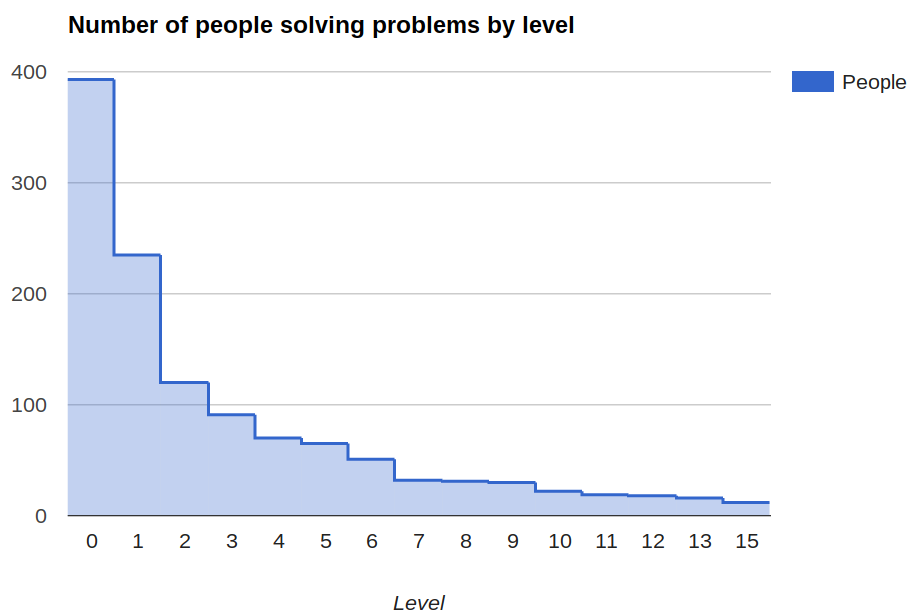
\includegraphics[width=\textwidth]{images/stats.png}
\caption{Stats by level.}
\label{fig:stats}
\end{figure}

Also, in table \ref{tab:ranking} is shown the top 15 people from the ranking, to this date. People with same number of problems are sorted by date of last problem solved.

\begin{table}[H]
\centering
  \begin{tabular}{| l || c |}
  \hline User & Current level  \\ \hline  \hline
gog & Finished  \\ \hline
cescmentation\_folch & Finished  \\ \hline
joseballester & Finished  \\ \hline
\begin{CJK}{UTF8}{min}すばらしい\end{CJK} & Finished  \\ \hline
dirbaio & Finished  \\ \hline
hermito & Finished  \\ \hline
davidalro & Finished  \\ \hline
gonzalo & Finished  \\ \hline
arbequi & Finished  \\ \hline
paualos3 & Finished  \\ \hline
Elfresh & Finished  \\ \hline
serk12 & Finished  \\ \hline
hydn & 14  \\ \hline
EducatedLobsters & 14  \\ \hline
albertvaka & 14  \\ \hline
  \end{tabular}
  \caption{Ranking with top 15.} \vspace{3pt}
  \label{tab:ranking}
\end{table}

\section{Feedback and more}
If you want to give some feedback about \texttt{The Game}, you can write us at the Facebook page \href{https://www.facebook.com/hackersatupc/}{Hackers at UPC}, share your opinion in the Facebook group \href{https://www.facebook.com/groups/hackersatupc/}{Hackers@UPC} or comment in our Slack Channel.

We hope you enjoyed participating in \texttt{The Game} as much as we did preparing it. See you at next HackUPC!
% ------------------------------------------------------------------------------
% End document
% ------------------------------------------------------------------------------
\end{document}